\section{FEM}

Der Vektorraum $\mathbb{V}$ hat undendlich viele Dimensionen. Falls wir n unabhängige Funktionen $v_1,\ldots,v_n$ wählen, dann spannen die Funktionen $a_1\cdot v_1(x)+\ldots+a_n\cdot v_n(x)$ einen n dimensionalen Teilraum $\mathbb{V}^{(n)}$  von $\mathbb{V}$ auf. Dabei gilt:\\

$\boxed{\tilde{u}^{(n)}=a_1\cdot v_1(x)+\ldots+a_n\cdot v_n(x)}$
\subsection{Das Verfahren von Ritz}
\textbf{Ritzsche Matrize: }
$R^{(n)}=\begin{bmatrix}
	R_{1,1}& R_{1,2}&\cdots\\
	R_{2,1}& R_{2,2}&\cdots\\
	\vdots & \vdots &\ddots\\
\end{bmatrix}$ \qquad mit \qquad $R_{j,k}^{(n)}=\int\limits_{0}^{1}{v_j'(x)\cdot
v_k'(x) dx}$\\
\textbf{Ritzscher Vektor: } 
$r^{(n)}=\begin{bmatrix}
	r_1\\
	r_2\\
	\vdots\\
\end{bmatrix}$ \qquad mit \qquad $r_{k}^{(n)}=\int\limits_{0}^{1}{f(x)\cdot v_k(x) dx}$\\

\textbf{Lösung nach Ritz:} $R^{(n)}\cdot a=r^{(n)}\qquad \Rightarrow \qquad a=\left\{R^{(n)}\right\}^{-1}\cdot r^{(n)}$
\subsection{Das Verfahren von Galerkin}
\textbf{Galerksche Matrize: }
$G^{(n)}=\begin{bmatrix}
	G_{1,1}& G_{1,2}&\cdots\\
	G_{2,1}& G_{2,2}&\cdots\\
	\vdots & \vdots &\ddots\\
\end{bmatrix}$ \qquad mit \qquad $G_{j,k}^{(n)}=\int\limits_{\partial \Omega}{\underbrace{(v_j''(x))}_{v_j \text{ in Form von DGL!}}\cdot v_k(x) dx}$\\
\textbf{Galerkscher Vektor: } 
$g^{(n)}=\begin{bmatrix}
	g_1\\
	g_2\\
	\vdots\\
\end{bmatrix}$ \qquad mit \qquad $g_{k}^{(n)}=\int\limits_{\partial \Omega}{f(x)\cdot v_k(x) dx}$\\

\textbf{Lösung nach Galerkin:} $G^{(n)}\cdot a+g^{(n)}=0\qquad \Rightarrow
\qquad a=\textcolor{red}{\mathbf{-}}\left\{G^{(n)}\right\}^{-1}\cdot g^{(n)}$\\

Die obige Matrix ist nur für die PDGL $-u''(x) = f(x)$ mit dem Ansatz
$\tilde{u}(x) = a_1 \cdot v_1(x) + a_2 \cdot v_2(x)$ gültig. Ansonsten muss ein
Gleichungssystem für $v_k$ = $v_1$ und $v_2$ aufgestellt werden (Beispiel
für DGL: $u''(x) + u(x) + x = 0$):\\
$\int\limits_{\partial \Omega}{(a_1 \cdot v_1'' + a_2 \cdot v_2'' + a_1 \cdot
v_1 + a_2 \cdot v_2 + x) \cdot v_k dx} = 0$

\subsection{Gewichtete Residuen}
\todo{Achtung: Gewichtete Residuen $\neq$ Bereichskollokation!! (Hinweis kann auch wieder gelöscht werden :) }

Gewichtungsfunktionen: $\{w_1(x),\ldots,w_n(x)\}$

\textbf{Matrize (gewichtete Residuen): }
$M^{(n)}=\begin{bmatrix}
	M_{1,1}& M_{1,2}&\cdots\\
	M_{2,1}& M_{2,2}&\cdots\\
	\vdots & \vdots &\ddots\\
\end{bmatrix}$ \qquad mit \qquad $M_{j,k}^{(n)}=\int\limits_{0}^{1}{v_j''(x)\cdot w_k(x) dx}$\\
\textbf{Vektor (gewichtete Residuen): } 
$m^{(n)}=\begin{bmatrix}
	m_1\\
	m_2\\
	\vdots\\
\end{bmatrix}$ \qquad mit \qquad $m_{k}^{(n)}=\int\limits_{0}^{1}{f(x)\cdot w_k(x) dx}$\\

\textbf{Lösung der gewichteten Residuen:} $M^{(n)}\cdot a+m^{(n)}=0\qquad \Rightarrow \qquad a=\textcolor{red}{\mathbf{-}}\left\{M^{(n)}\right\}^{-1}\cdot m^{(n)}$

\subsection{Punktkollokation}
Im Sinne einer Punktkollokation (einzelne Punkte müssen zwischen wahrem Resultat und Approximation übereinstimmen) werden $n$ Stützstellen im Intervall von $[0,1]$ gewählt.\\

$\begin{bmatrix}
	v_1''(x_1)& v_2''(x_1)&\cdots\\
	v_1''(x_2)& v_2''(x_2)&\cdots\\
	\vdots& \vdots&\ddots
\end{bmatrix}\cdot
\begin{bmatrix}
a_1\\
a_2\\
\vdots
\end{bmatrix}
=\begin{bmatrix}
-f(x_1)\\
-f(x_2)\\
\vdots
\end{bmatrix}$\qquad Das Gleichungssystem nach a auflösen\\

Die obige Matrix ist nur für die PDGL $-u''(x) = f(x)$ mit dem Ansatz
$\tilde{u}(x) = a_1 \cdot v_1(x) + a_2 \cdot v_2(x)$ gültig. Ansonsten muss die
DGL mit den Ansatzfunktionen aufgestellt und an beiden Punkten eingesetzt
werden, um $a_1$ und $a_2$ zu bestimmen:\\
DGL: $u''(x) + u(x) + x = 0$ $\Rightarrow$ Gleichung an Punkt 1: $a_1 \cdot
v_1''(x_1) + a_2 \cdot v_2''(x_1) + a_1 \cdot v(x_1) + a_2 \cdot v(x_1) + x_1 =
0$




\subsection{Bereichskollokation}
Im Gegensatz zur Punktkollokation müssen nicht einzelne Punkte sondern ganze Bereiche (Intervalle $I_k$) übereinstimmen. Für $-u''(x) = f(x)$ wird dieses Gleichungssystem aufgestellt.

$\begin{bmatrix}
	\int_{I_1} v_1'' & \int_{I_1} v_2''& \cdots\\
	\int_{I_2} v_1'' & \int_{I_2} v_2''& \cdots\\
	\vdots& \vdots&\ddots
\end{bmatrix}\cdot
\begin{bmatrix}
a_1\\
a_2\\
\vdots
\end{bmatrix}
=\begin{bmatrix}
-\int_{I_1} f(x)\\
-\int_{I_2} f(x)\\
\vdots
\end{bmatrix}$\qquad Das Gleichungssystem nach a auflösen


\subsection{Das Verfahren von Gauss (MSE)}

\textbf{Gausscher Matrize: }
$Q^{(n)}=\begin{bmatrix}
	Q_{1,1}& Q_{1,2}&\cdots\\
	Q_{2,1}& Q_{2,2}&\cdots\\
	\vdots & \vdots &\ddots\\
\end{bmatrix}$ \qquad mit \qquad $Q_{j,k}^{(n)}=\int\limits_{0}^{1}{v_j''(x)\cdot v_k''(x) dx}$\\
\textbf{Gausscher Vektor: } 
$q^{(n)}=\begin{bmatrix}
	q_1\\
	q_2\\
	\vdots\\
\end{bmatrix}$ \qquad mit \qquad $q_{k}^{(n)}=\int\limits_{0}^{1}{f(x)\cdot v_k''(x) dx}$\\

\textbf{Lösung nach Gauss:} $Q^{(n)}\cdot a+q^{(n)}=0\qquad \Rightarrow \qquad a=\textcolor{red}{\mathbf{-}}\left\{Q^{(n)}\right\}^{-1}\cdot q^{(n)}$

\subsection{Finite Elemente}

Die besprochenen Verfahren setzen die Wahl eines Satzes $v_1(x),\ldots,v_n(x)$ von Grundfunktionen voraus. Bei FEM wird mit lokalen Trägern (Grundfunktionen) gearbeitet, diese sind nur auf einem kleinen Intervall ungleich null. Der Vorteil dieses Vorgehens liegt darin, dass in einem Bereich nur ein Träger die Approximationsfunktion beeinflusst. Der Nachteil liegt in der hohen Anzahl der so benötigten Träger.\\

\textbf{WICHTIG:} Alle Verfahren werden mit einer Diskretisierung von $h=1/3$
vorgestellt.

\subsubsection{Knotenvariablen}
Als erstes werden auf dem Intervall $[0,1]$ $n$, normalerweise gleichverteilte, Knotenstellen eingeführt.

\begin{minipage}{11cm}
Dadurch wird das Intervall $[0,1]$ in Teilintervalle (Maschen) zerlegt.\\
 
Für $n=3$:\quad $I_1=[0,1/3]$\quad $I_1=[1/3,2/3]$\quad $I_1=[2/3,1]$\\

Als nächstes wird jeder Knotenstelle $x_k$ eine Ansatzvariable (Knotenvariable) zugeordnet.\\

Ansatz: \quad $\tilde{u}(0)=a_0$\quad $\tilde{u}(1/3)=a_1$\quad $\tilde{u}(2/3)=a_2$\quad $\tilde{u}(1)=a_3$\\

Zusatzbedingungen:
\begin{tabular}{llll}
$v_0(0)=1$&$v_0(1/3)=0$&$v_0(2/3)=0$&$v_0(1)=0$\\
$v_1(0)=0$&$v_1(1/3)=1$&$v_1(2/3)=0$&$v_1(1)=0$\\
$v_2(0)=0$&$v_2(1/3)=0$&$v_2(2/3)=1$&$v_2(1)=0$\\
$v_3(0)=0$&$v_3(1/3)=0$&$v_3(2/3)=0$&$v_3(1)=1$\\
\end{tabular}
\end{minipage}
\hfill
\begin{minipage}{8cm}
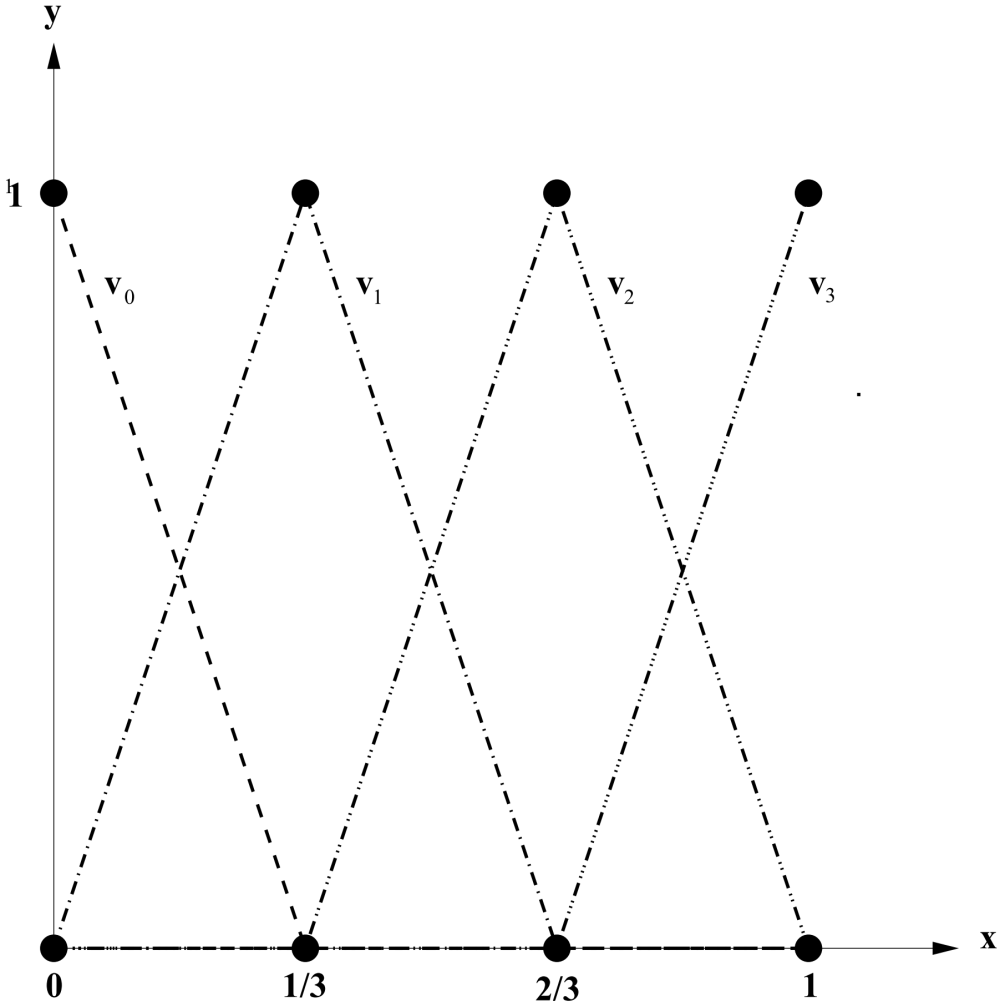
\includegraphics[width=8cm]{Content/Numerik/Traeger1.png}
\end{minipage}


\subsubsection{Formfunktionen}
Die lokalen Grundfunktionen sollen aus Teilstücken einfacher Funktionen, z.B: Polynomen, die nur auf einer einzelnen Masche definiert sind zusammengesetzt werden.\\
Zwei mögliche Formfunktionen sind Beispielsweise:\quad $l_1(x)=1-x$\quad und \quad $l_2(x)=x$\\

\begin{minipage}{8cm}
	\begin{tabular}{lc|c|c}
	$t\in$&$[0,1/3]$&$[1/3,2/3]$&$[2/3,1]$\\
	\hline
	$v_0=$&$1-3x$&$0$&$0$\\
	$v_1=$&$3x$&$2-3x$&$0$\\
	$v_2=$&$0$&$-1+3x$&$3-3x$\\
	$v_3=$&$0$&$0$&$-2+3x$\\
	\end{tabular}
\end{minipage}
\hfill
\begin{minipage}{2cm}
$\Longrightarrow$
\end{minipage}
\hfill
\begin{minipage}{8cm}
	\begin{tabular}{lc|c|c}
	$t\in$&$[0,1/3]$&$[1/3,2/3]$&$[2/3,1]$\\
	\hline
	$v_0=$&$l_1(3x)$&$0$&$0$\\
	$v_1=$&$l_2(3x)$&$l_1(3x-1)$&$0$\\
	$v_2=$&$0$&$l_2(3x-1)$&$l_1(3x-2)$\\
	$v_3=$&$0$&$0$&$l_2(3x-2)$\\
	\end{tabular}
\end{minipage}
\subsubsection{Elementmatrizen}
Grundsätzlich kann die Ansatzvariable durch jedes Verfahren bestimmt werden.
Weil bei einer linearen Ansatzfunktion die zweite Ableitung trivial $(=0)$ ist die Wahl des Ritzschen Verfahren erzwungen.

Die Integrale werden maschenweise ausgewertet:\\

 $\int\limits_{0}^{1}{}=\int\limits_{0}^{1/3}{}+\int\limits_{1/3}^{2/3}{}+\int\limits_{2/3}^{1}{}$\\
 
Durch diesen Ansatz wird die Ritzsche Matrize über jede Masche einzeln berechnet und danach zur globalen Ritzschen Matrize aufsummier:\\

\qquad $R^{(4)}=R^{(4,1)}+R^{(4,2)}+R^{(4,3)}=
\begin{bmatrix}
	* & * & 0 & 0\\
	* & * & 0 & 0\\
	0 & 0 & 0 & 0\\
	0 & 0 & 0 & 0\\
\end{bmatrix}+
\begin{bmatrix}
	0 & 0 & 0 & 0\\
	0 & * & * & 0\\
	0 & * & * & 0\\
	0 & 0 & 0 & 0\\
\end{bmatrix}+
\begin{bmatrix}
	0 & 0 & 0 & 0\\
	0 & 0 & 0 & 0\\
	0 & 0 & * & *\\
	0 & 0 & * & *\\
\end{bmatrix}
$\\

Die mit $*$ bezeichneten $2\times 2$ Matrizen heissen Maschenmatrizen:\\

$M^{(4,1)}=M^{(4,2)}=M^{(4,3)}=
\begin{bmatrix}
	* & *\\
	* & *\\
\end{bmatrix}=3\cdot\begin{bmatrix}
	-1 & 1\\
	1 & -1\\
\end{bmatrix}\qquad\Rightarrow\qquad\boxed{M=\frac 1h\cdot
\underset{\text{\textbf{E}: Elementmatrize}}{\underbrace{\begin{bmatrix}
	-1 & 1\\
	1 & -1\\
\end{bmatrix}}}=\frac 1h\cdot \mathbf{E}}$\\

Die Elementmatrize wird nun in die entsprechende Ritzsche Matrize eingesetzt und überlagert. Für die Quantisierung von $h=1/3$ ergibt sich:\\

$R^{4}=
\begin{bmatrix}
	-3 & 3 & 0 & 0 \\
	3 & -3-3 & 3 & 0 \\
	0 & 3 & -3-3 & 3 \\
	0 & 0 & 3 & -3 \\
\end{bmatrix}=
\begin{bmatrix}
	-3 & 3 & 0 & 0 \\
	3 & -6 & 3 & 0 \\
	0 & 3 & -6 & 3 \\
	0 & 0 & 3 & -3 \\
\end{bmatrix}$\\

Der Ritzsche Vektor muss mittels Integration berechnet werden:\\

$r^4=
\begin{bmatrix}
	\int\limits_{0}^{1}{f(x)\cdot v_0(x)dx}\\
	\int\limits_{0}^{1}{f(x)\cdot v_1(x)dx}\\
	\int\limits_{0}^{1}{f(x)\cdot v_2(x)dx}\\
	\int\limits_{0}^{1}{f(x)\cdot v_3(x)dx}\\
\end{bmatrix}$\\

Das Ritzsche Gleichungssystem dazu ist: $\boxed{R^4\cdot a+r^4=0} \qquad\Rightarrow\qquad a=-\left\{R^4\right\}^{-1}\cdot r^4$\\

\textbf{Anfangsbedingungen:} Die Anfangsbedingungen $a_0$ und $a_n$ können direkt eingesetzt werden.\\

$a_0=10$\qquad$a_3=20$\\

$
	\begin{bmatrix}
		3 & -6 & 3 & 0 \\
		0 & 3 & -6 & 3 \\
	\end{bmatrix}\cdot
	\begin{bmatrix}
		10\\a_1\\a_2\\20
	\end{bmatrix}+r^4=0\qquad\Rightarrow\qquad
	\begin{bmatrix}
		-6 & 3 \\
		 3 & -6 \\
	\end{bmatrix}\cdot
	\begin{bmatrix}
		a_1\\a_2
	\end{bmatrix}+
	\begin{bmatrix}
		30\\60
	\end{bmatrix}+
	r^4=0
$\\

$
	\begin{bmatrix}
			a_1\\a_2
	\end{bmatrix}=
	\begin{bmatrix}
		-6 & 3 \\
	 	 3 & -6 \\
	\end{bmatrix}^{-1}\cdot
	\begin{bmatrix}
		-\left(r^4_1+3\cdot a_0\right)\\
		-\left(r^4_2+3\cdot a_3\right)\\
	\end{bmatrix}		
$

\subsubsection{Die Finite Elemente Handrechnung}
\textbf{Problemstellung:} $u''(x)+f(x)=0\qquad f(x)=20\qquad u(0)=10\qquad u(1)=20$\\

Die Approximation soll auf den \textbf{NICHT} gleichverteilten Intervallen: $[0,1/6]$,\quad $[1/6,1/2]$,\quad $[1/2,1]$\\

Die Entsprechenden Elementmatrizen E sind:\\

$
	\frac{1}{1/6}\begin{bmatrix}
		-1 & 1\\
		1 & -1
	\end{bmatrix}=
	\begin{bmatrix}
			-6 & 6\\
			6 & -6
	\end{bmatrix}\qquad
	\frac{1}{1/2-1/6}\begin{bmatrix}
		-1 & 1\\
		1 & -1
	\end{bmatrix}=
	\begin{bmatrix}
		-3 & 3\\
		3 & -3
	\end{bmatrix}\qquad
	\frac{1}{1-1/2}\begin{bmatrix}
		-1 & 1\\
		1 & -1
	\end{bmatrix}=
	\begin{bmatrix}
		-2 & 2\\
		2 & -2
	\end{bmatrix}
$\\
\\

\begin{minipage}{10cm}
Der Ritzsche Vektor und die Ritzsche Matrize sind:\\

$R^n=
\begin{bmatrix}
		-6 & 6 & 0 & 0\\
		6 & -9 & 3 & 0\\
		0 & 3 & -5 & 2\\
		0 & 0 & 2 & -2\\
\end{bmatrix}$

$
r^n=\begin{bmatrix}
		\int\limits_{0}^{1/6}{f(x)\cdot(1-6x)}dx\\
		\int\limits_{0}^{1/6}{f(x)\cdot(6x)}+\int\limits_{1/6}^{3/6}{f(x)\cdot(3/2-3x)}dx\\
		\int\limits_{1/6}^{3/6}{f(x)\cdot(3x-1/2)}+\int\limits_{3/6}^{1}{f(x)\cdot(2-2x)}dx\\
		\int\limits_{1/2}^{1}{f(x)\cdot(2x-1)}dx\\
\end{bmatrix}=
\begin{bmatrix}
	5/3\\
	5\\
	25/3\\
	5
\end{bmatrix}
$\end{minipage}
\hfill
\begin{minipage}{9cm}
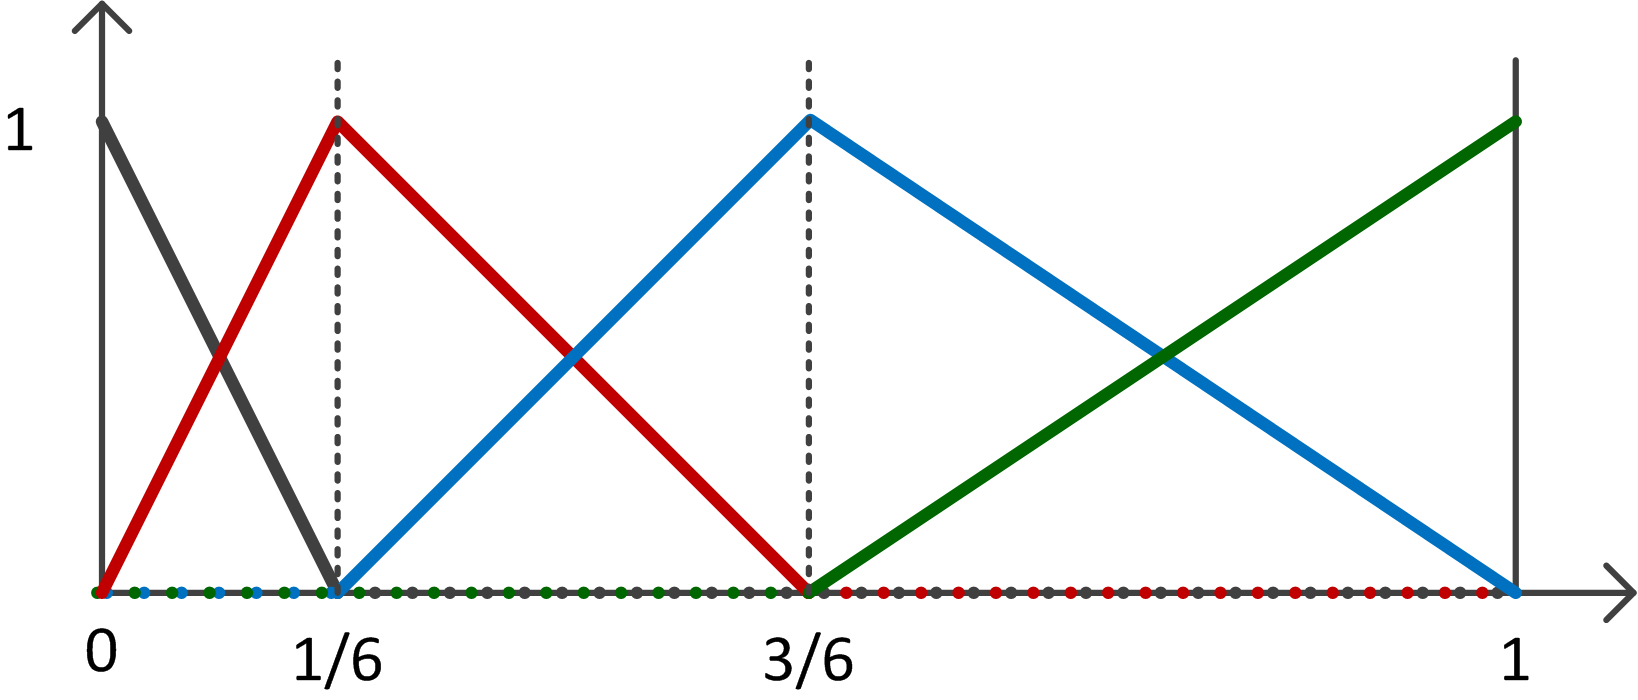
\includegraphics[width=9cm]{Content/Numerik/FEMHand}
\end{minipage}\\

$R^n\cdot a +r^n=0 \qquad\Rightarrow\qquad
\begin{bmatrix}
	-6 & 6 & 0 & 0\\
	6 & -9 & 3 & 0\\
	0 & 3 & -5 & 2\\
	0 & 0 & 2 & -2\\
\end{bmatrix}\cdot
\begin{bmatrix}
	10\\
	a_1\\
	a_2\\
	20
\end{bmatrix}+
\begin{bmatrix}
	5/3\\
	5\\
	25/3\\
	5
\end{bmatrix}=
\begin{bmatrix}
	0\\
	0\\
	0\\
	0
\end{bmatrix}\qquad\Rightarrow\qquad
\begin{bmatrix}
	6 & -9 & 3 & 0\\
	0 & 3 & -5 & 2\\
\end{bmatrix}\cdot
\begin{bmatrix}
	10\\
	a_1\\
	a_2\\
	20
\end{bmatrix}+
\begin{bmatrix}
	5/3\\
	5\\
	25/3\\
	5
\end{bmatrix}=
\begin{bmatrix}
	0\\
	0\\
	0\\
	0
\end{bmatrix}	
$\\
\\

$\qquad\Rightarrow\qquad
\begin{bmatrix}
	-9 & 3\\
	3 & -5\\
\end{bmatrix}\cdot
\begin{bmatrix}
	a_1\\
	a_2\\
\end{bmatrix}+
\begin{bmatrix}
	6\cdot 10\\
	2\cdot 20\\
\end{bmatrix}+
\begin{bmatrix}
	5\\
	25/3\\
\end{bmatrix}
=0\qquad\Rightarrow\qquad
\begin{bmatrix}
	-9 & 3\\
	3 & -5\\
\end{bmatrix}\cdot
\begin{bmatrix}
	a_1\\
	a_2\\
\end{bmatrix}=
\begin{bmatrix}
	-65\\
	-145/3\\
\end{bmatrix}\qquad\Rightarrow\qquad
\begin{bmatrix}
	a_1\\
	a_2\\
\end{bmatrix}=
\begin{bmatrix}
	235/18\\
	35/2\\
\end{bmatrix}
$\\
\\
$
\qquad\Rightarrow\qquad \tilde{u}(x)=10\cdot v_0(x)+\frac{235}{18} v_1(x)+\frac{35}{2}\cdot v_2(x)+20\cdot v_3(x)=
$




\subsubsection{h-Strategie}

Die Grundidee der h-Strategie ist die Verfeinerung der Auflösung. Mit anderen Worten die Maschenbreite $h$ wird verkleinert. Um den ganzen Bereich dennoch abdecken zu können sind mehr Maschen notwendig.

\subsubsection{p-Strategie}
Bei der p-Strategie bleibt das Netz bestehen. Die Ansatzfunktionen sollen nun durch Polynome höherer Ordnung zusammengesetzt werden, dazu werden neue Knoten und Knotenvariablen eingeführt werden.\\

\textbf{Problemstellung:} $u''(x)+f(x)=0\qquad u(0)=a_0\qquad u(1)=a_6$\\

Die Approximation soll auf dem gleichverteilten Intervallen gelten: $[0,1/3]$,\quad $[1/3,2/3]$,\quad $[2/3,1]$\\

\begin{minipage}{4cm}
	Formfunktionen:\\

	$q_1(x)=(1-x)\cdot(1-2x)$\\
	$q_2(x)=4x\cdot(1-x)$\\
	$q_3(x)=-x\cdot(1-2x)$\\
	
	Elementmatrize: $\boxed{E=\frac{1}{h}
	\begin{bmatrix}
		-7& 8 & -1\\
		8& -16& 8\\
		-1& 8& -7	
	\end{bmatrix}}$\\
\end{minipage}
\hfill
\begin{minipage}{8cm}
	\begin{tabular}{lc|c|c}
		$x\in$&$[0,1/3]$&$[1/3,2/3]$&$[2/3,1]$\\
		\hline
		$v_0=$&$q_1(3x)$&$0$&$0$\\
		$v_1=$&$q_2(3x)$&$0$&$0$\\
		$v_2=$&$q_3(3x)$&$q_1(3x-1)$&$0$\\
		$v_3=$&$0$&$q_2(3x-1)$&$0$\\
		$v_4=$&$0$&$q_3(3x-1)$&$q_1(3x-2)$\\
		$v_5=$&$0$&$0$&$q_2(3x-2)$\\
		$v_6=$&$0$&$0$&$q_3(3x-2)$\\
	\end{tabular}
\end{minipage}
\hfill
\begin{minipage}{6cm}
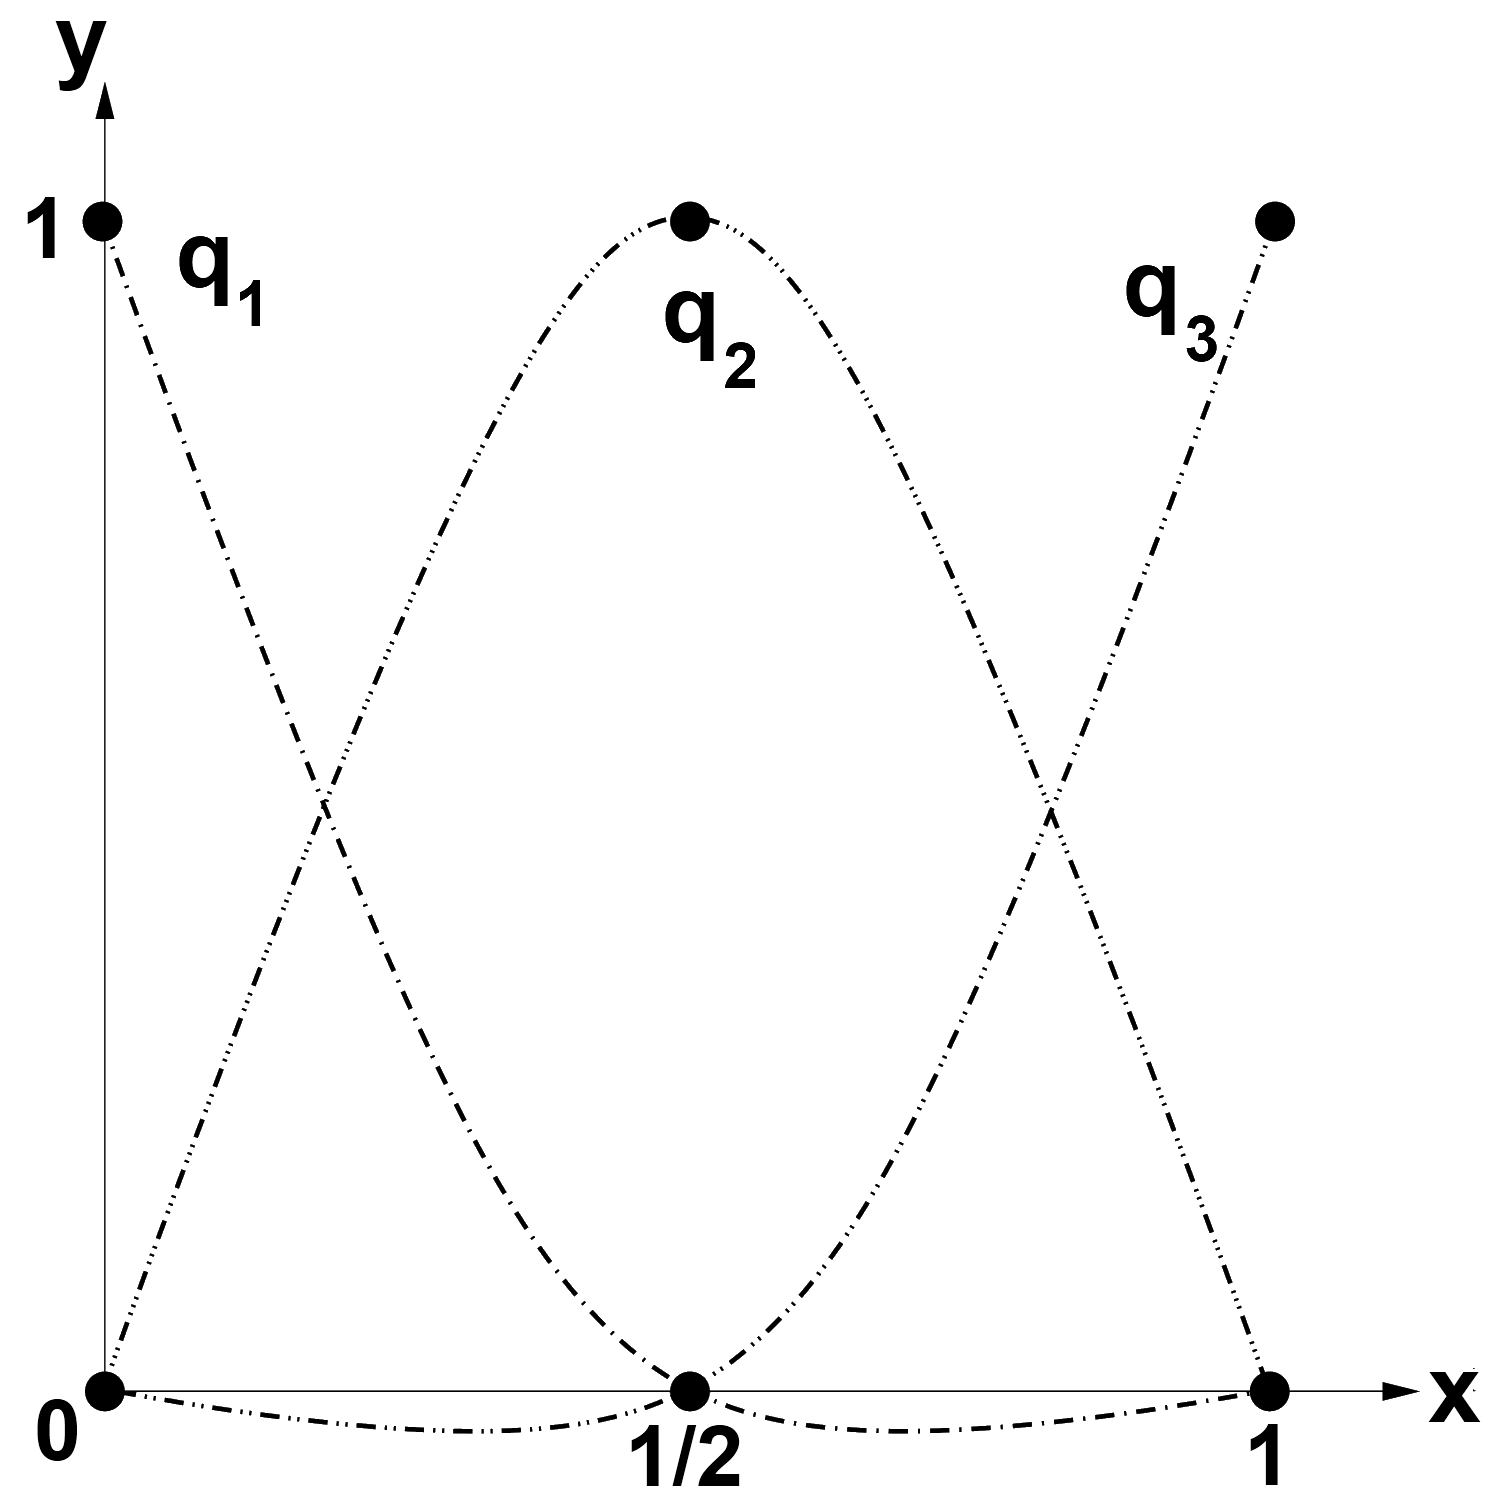
\includegraphics[width=6cm]{Content/Numerik/FEM2Ord}
\end{minipage}\\

$\underset{\text{Ritzsche Matrize $R^{(8)}$ für } h=1/3}{\underbrace{3\begin{bmatrix}
	-7& 8 & -1& 0& 0& 0& 0\\
	 8& -16& 8& 0& 0& 0& 0\\
	-1& 8& -14& 8& -1& 0& 0\\ 
	 0& 0& 8& -16& 8& 0& 0\\
	 0& 0& -1& 8& -14& 8& -1\\ 
	 0& 0& 0& 0& 8& -16& 8\\
	 0& 0& 0& 0& -1& 8& -7	
\end{bmatrix}}}\cdot\begin{bmatrix}
	a_0\\
	a_1\\
	a_2\\
	a_3\\
	a_4\\
	a_5\\
	a_6\\
\end{bmatrix}
+\underset{\text{Ritzscher Vektor $r^{(8)}$ für } h=1/3}{\underbrace{\begin{bmatrix}
	\int\limits_{0}^{1}{f(x)\cdot v_0(x)dx}\\
	\int\limits_{0}^{1}{f(x)\cdot v_1(x)dx}\\
	\int\limits_{0}^{1}{f(x)\cdot v_2(x)dx}\\
	\int\limits_{0}^{1}{f(x)\cdot v_3(x)dx}\\
	\int\limits_{0}^{1}{f(x)\cdot v_4(x)dx}\\
	\int\limits_{0}^{1}{f(x)\cdot v_5(x)dx}\\
	\int\limits_{0}^{1}{f(x)\cdot v_6(x)dx}\\
\end{bmatrix}}}=
\begin{bmatrix}
	0\\
	0\\
	0\\
	0\\
	0\\
	0\\
	0\\
	0\\
\end{bmatrix}
$\\

\textbf{Vorteil der p-Strategie gegenüber der h-Strategie:} Bei beiden Strategien steigt die Dimension der Systemmatrizen an. Es besteht jedoch die berechtigte Hoffnung, dass der Zuwachs der benötigt wird, um eine vergleichbare Genauigkeit zu errreichen, bei der p-Strategie weitaus geringer ist als bei der h-Strategie. 

\subsection{Konformität und Vollständigkeit}
Muss nun die Approximationslösung zweimal ableitbar sein, so gilt der Ansatz des letzten Abschnitt nicht mehr als konform.

Um die einmalige Differenzierbarkeit an den Knoten zu gewährleisten müssen neue Grundfunktionen gefunden werden.\\

$\tilde{u}(x)=a_0v_0(x)+a_1v_1(x)+a_2v_2(x)+a_3v_3(x)+\tilde{a}_0\tilde{v}_0(x)+\tilde{a}_1\tilde{v}_1(x)+\tilde{a}_2\tilde{v}_2(x)+\tilde{a}_3\tilde{v}_3(x)$\\

Zwei Grundfunktionen stellen den richtigen Wert and den Knoten sicher. Zwei weitere Grundfunktionen werden benötigt um die erste Ableitung (Steigung) an den Übergangknoten sicherzustellen, sie sorgen für die Vollständigkeit der Grundfunktionen. (Ohne die zwei weiteren Grundfunktionen wäre an den Übergangsknoten nur eine Steigung von Null möglich.)

\subsection{Hermetische Polynome dritter Ordnung}
Übereinstimmung bis zur 1.Ableitung an den Knotenpunkten\\

\textbf{Problemstellung:} $u''(x)+f(x)=0\qquad u(0)=a_0\qquad u'(0)=\tilde{a}_0 \qquad u(1)=a_3\qquad  u'(1)=\tilde{a}_3$\\

Die Approximation soll auf dem gleichverteilten Intervallen gelten: $[0,1/3]$,\quad $[1/3,2/3]$,\quad $[2/3,1]$\\

\begin{minipage}{4cm}
Formfunktionen:\\
$h_1(x)=2t^3-3t^2+1$\\
$h_2(x)=t^3-2t^2+t$\\
$h_3(x)=-2t^3+3t^2$\\
$h_4(x)=t^3-t^2$
\end{minipage}
\hfill
\begin{minipage}{8cm}
	\begin{tabular}{lc|c|c}
		$x\in$&$[0,1/3]$&$[1/3,2/3]$&$[2/3,1]$\\
		\hline
		$v_0=$&$h_1(3x)$&$0$&$0$\\
		$\tilde{v}_0=$&$\frac 13 h_2(3x)$&$0$&$0$\\
		$v_1=$&$h_3(3x)$&$h_1(3x-1)$&$0$\\
		$\tilde{v}_1=$&$\frac 13 h_4(3x)$&$\frac 13 h_2(3x-1)$&$0$\\
		$v_2=$&$0$&$h_3(3x-1)$&$h_1(3x-2)$\\
		$\tilde{v}_2=$&$0$&$\frac 13 h_4(3x-1)$&$\frac 13 h_2(3x-2)$\\
		$v_3=$&$0$&$0$&$h_3(3x-2)$\\
		$\tilde{v}_3=$&$0$&$0$&$\frac 13 h_2(3x-1)$\\
	\end{tabular}
\end{minipage}
\hfill
\begin{minipage}{6cm}
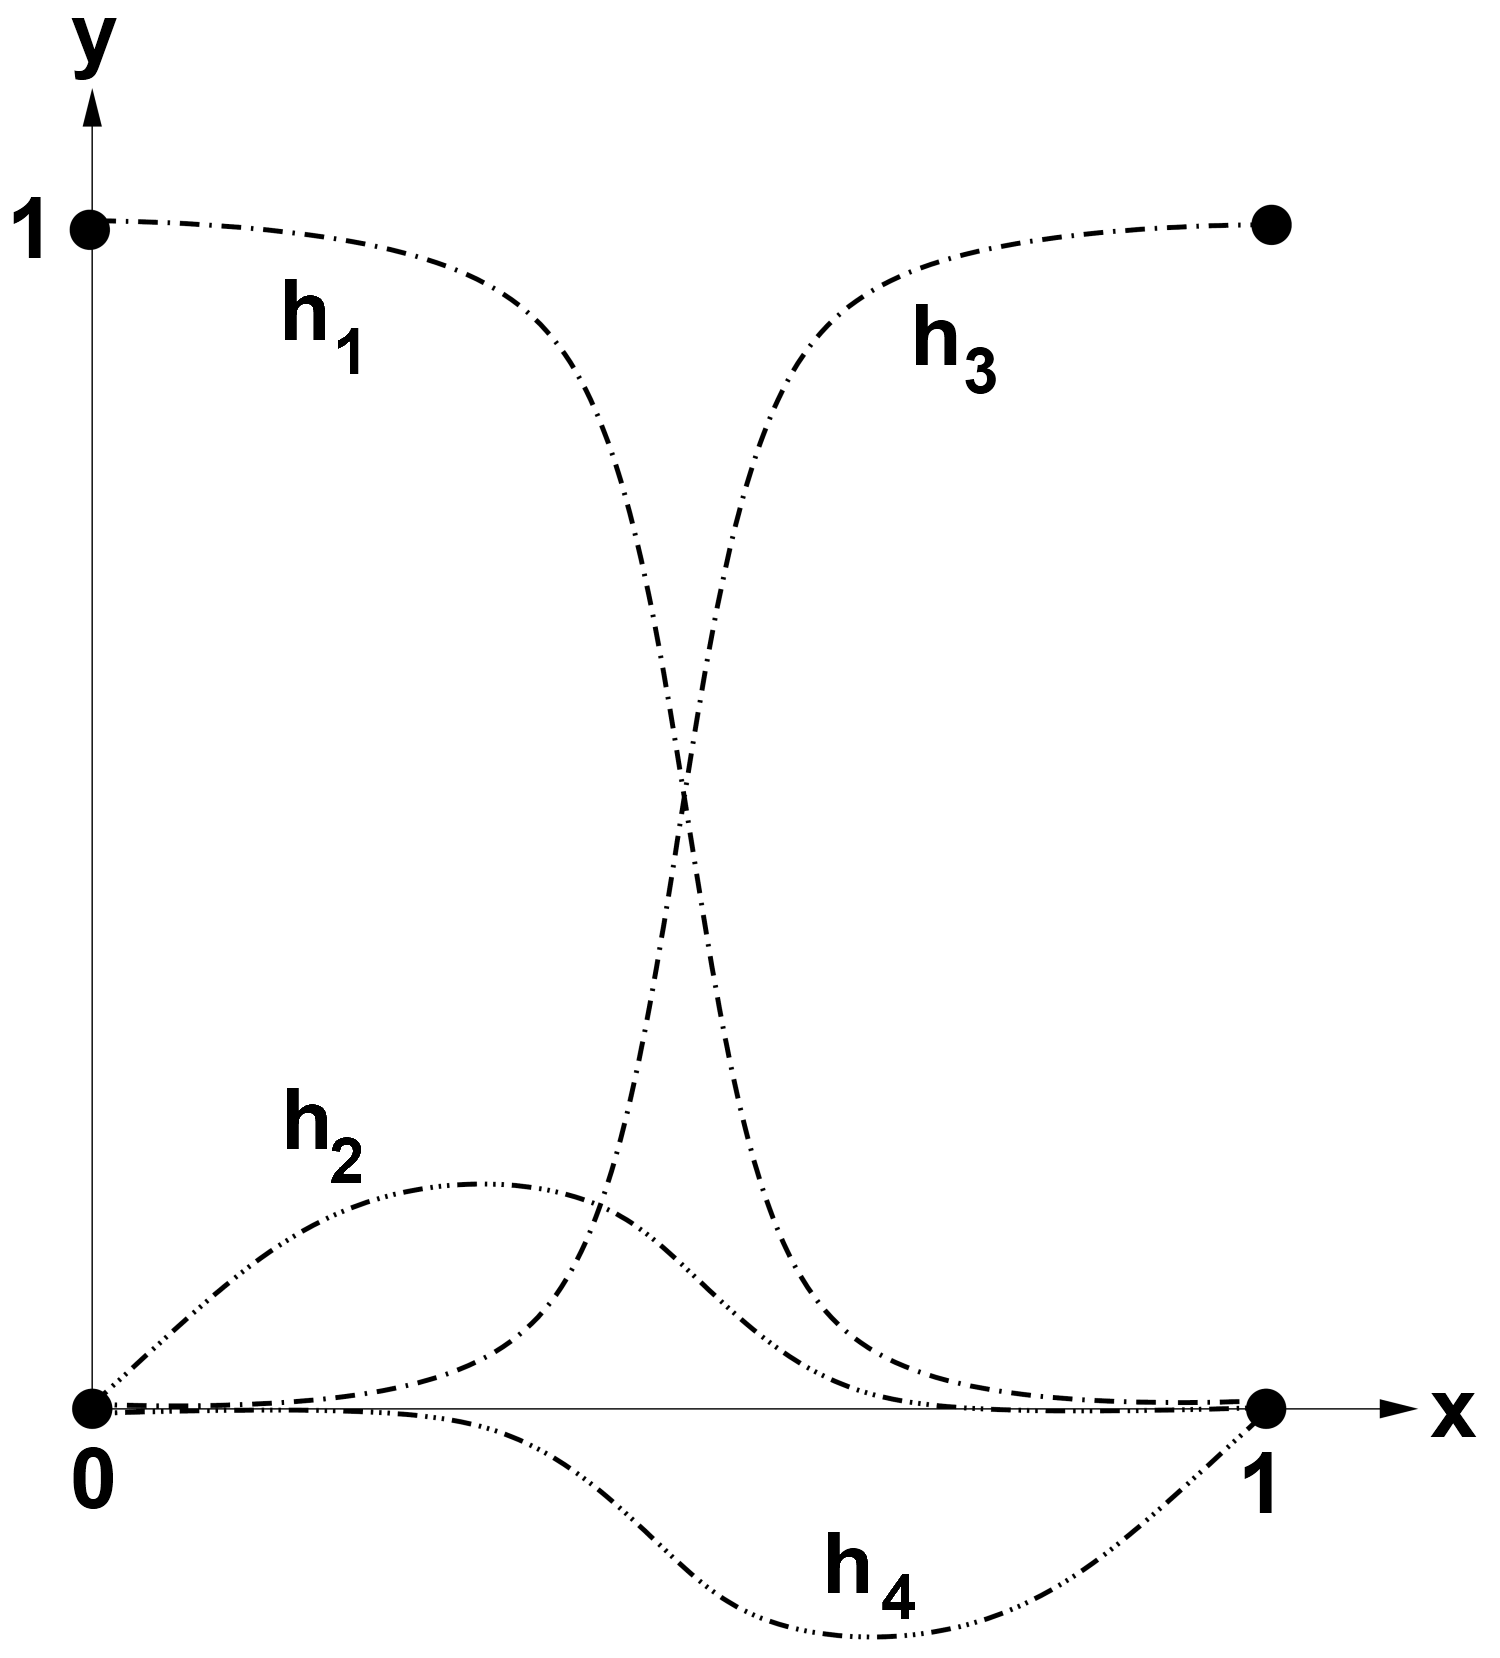
\includegraphics[width=6cm]{Content/Numerik/FEM3Ord}
\end{minipage}\\
$E=\frac{1}{30}
\begin{bmatrix}
	-36 & -3 & 36 & -3\\
	-3 & -4 & 3 & 1\\
	36 & 3 & -36 & 3\\
	-3 & 1 & 3 & -4\\
\end{bmatrix}\qquad\Rightarrow\qquad
\boxed{M=\frac{1}{30\cdot h}
\begin{bmatrix}
	-36 & -3\cdot h & 36 & -3\cdot h\\
	-3\cdot h & -4\cdot h^2 & 3\cdot h & 1\cdot h^2\\
	36 & 3\cdot h & -36 & 3\cdot h\\
	-3\cdot h & 1\cdot h^2 & 3\cdot h & -4\cdot h^2\\
\end{bmatrix}}$\\
\\


$\underset{\text{Ritzsche Matrize $R^{(8)}$ für } h=1/3}{\underbrace{\frac{3}{30}\begin{bmatrix}
	-36 & -1 & 36 & -1 & 0  & 0  & 0  & 0 \\
	-1  & -4/9  & 1  & 1/9  & 0  & 0  & 0  & 0\\
	36  & 1  & -72  & 0  & 36  & -1  & 0  & 0\\
	-1  & 1/9  & 0  & -8/9  & 1  & 1/9  & 0  & 0\\
	0  & 0  & 36  & 1  & -72  & 0  & 36  & -1\\
	0  & 0  & -1  & 1/9  & 0  & -8/9  & 1  & 1/9\\
	0  & 0  & 0  & 0  & 36  & 1  & -36  & 1\\
	0  & 0  & 0  & 0  & -1  & 1/9  & 1  & -4/9\\
\end{bmatrix}}}\cdot\begin{bmatrix}
	a_0\\
	\tilde{a}_0\\
	a_1\\
	\tilde{a}_1\\
	a_2\\
	\tilde{a}_2\\
	a_3\\
	\tilde{a}_3\\
\end{bmatrix}
+\underset{\text{Ritzscher Vektor $r^{(8)}$ für } h=1/3}{\underbrace{\begin{bmatrix}
	\int\limits_{0}^{1}{f(x)\cdot v_0(x)dx}\\
	\int\limits_{0}^{1}{f(x)\cdot \tilde{v}_0(x)dx}\\
	\int\limits_{0}^{1}{f(x)\cdot v_1(x)dx}\\
	\int\limits_{0}^{1}{f(x)\cdot \tilde{v}_1(x)dx}\\
	\int\limits_{0}^{1}{f(x)\cdot v_2(x)dx}\\
	\int\limits_{0}^{1}{f(x)\cdot \tilde{v}_2(x)dx}\\
	\int\limits_{0}^{1}{f(x)\cdot v_3(x)dx}\\
	\int\limits_{0}^{1}{f(x)\cdot \tilde{v}_3(x)dx}\\
\end{bmatrix}}}=
\begin{bmatrix}
	0\\
	0\\
	0\\
	0\\
	0\\
	0\\
	0\\
	0\\
\end{bmatrix}
$\\







%\subsection{FEM für parabolische PDEs}